%-----------------------------------------------------------
%   Capítulo 8 - Conclusão e Trabalho Futuro
%-----------------------------------------------------------
\chapter{Conclusão e Trabalho Futuro}

Os resultados obtidos com este projeto são bastante satisfatórios, pois consegui-se ter um sistema totalmente funcional e a medir valores razoáveis.
No geral os principais objetivos foram atingidos, nomeadamente, todos os 8 sensores estão funcionais , calcular o \textit{roll} e comunicar utilizando o protocolo definido pelo \textit{master}.

\section{Trabalhos futuros}
Como trabalhos futuros, o protótipo poderia ser reformulado para um novo \textit{design}, que está na figura \ref{new}, pois se fossem utilizados dois anéis (círculos a preto) para medir roll e três tiras (retas a vermelho) que iriam medir o pich, seriam eliminados alguns problemas, pois os anéis com a medição do roll definiriam qual a tira que iria enviar o pitch, deixando de existir tanta dependência dos da normalização dos sensores.  

\begin{figure}[!htb]
\centering
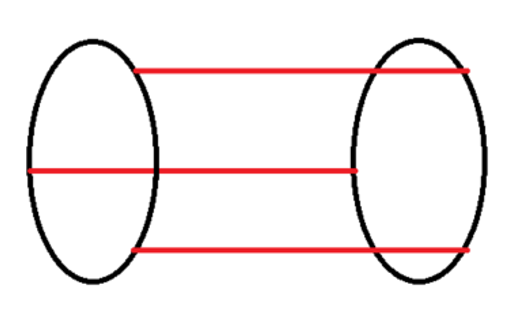
\includegraphics[scale=0.7]{Figuras/new.PNG}
\caption{Possível reformulação das posições dos sensores}
\label{new}
\end{figure}